\chapter{Тактовый генератор}

\begin{center}
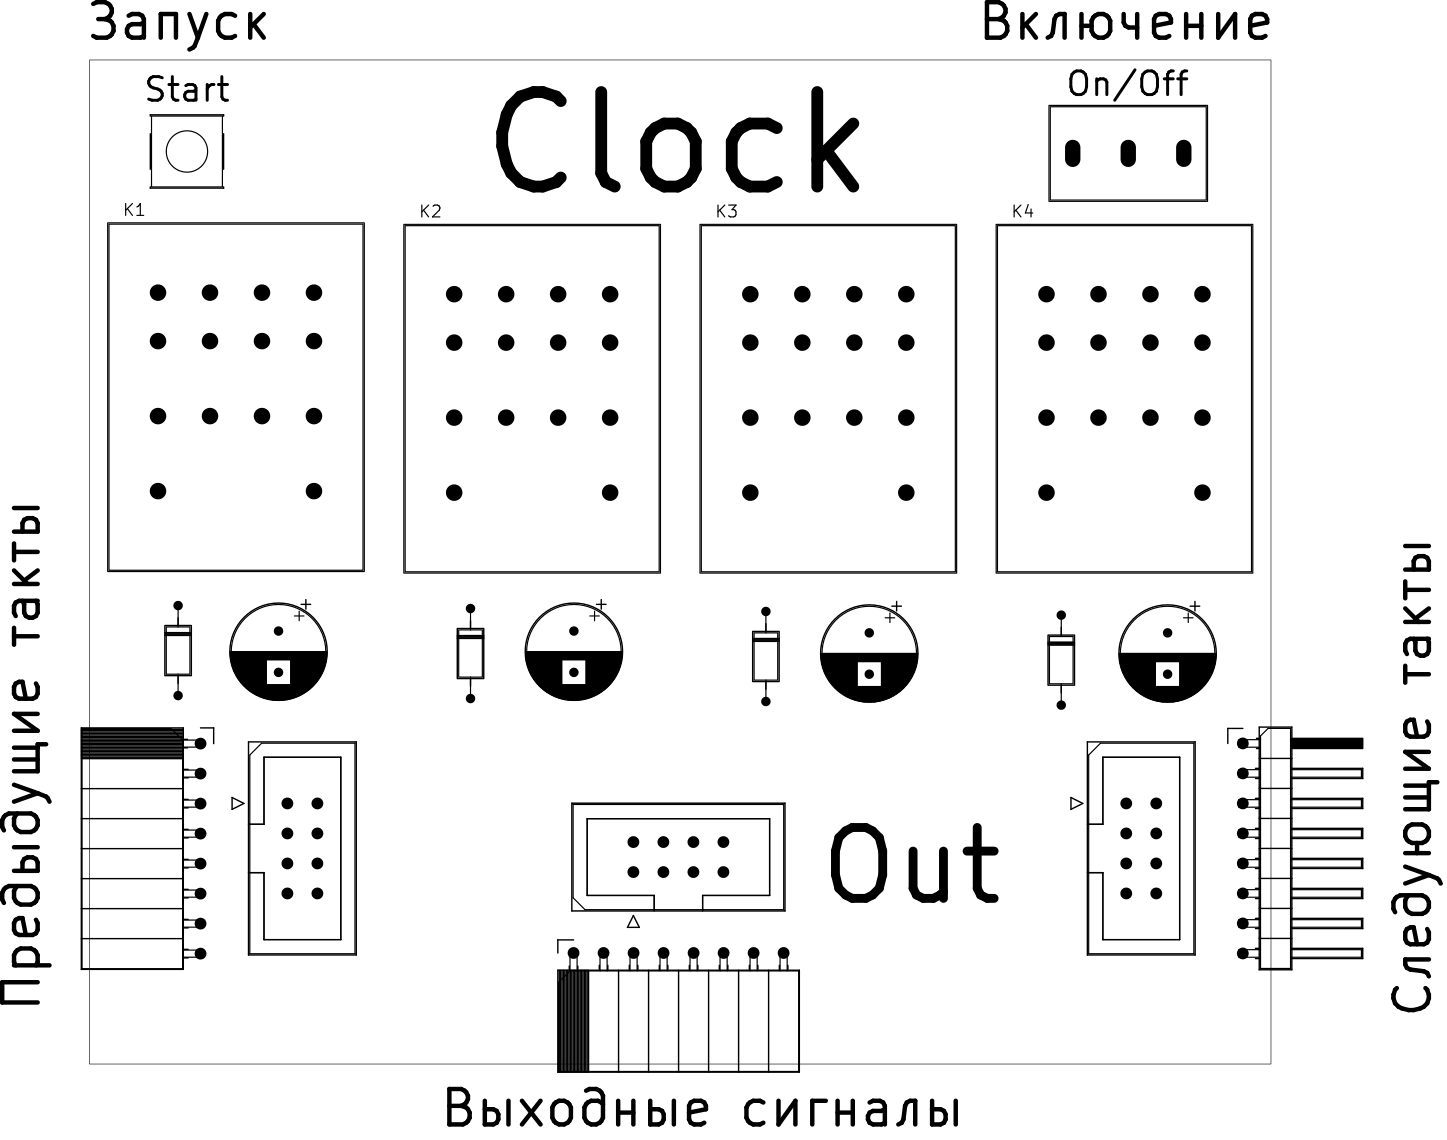
\includegraphics{../modules-png/clock-pcb.png}
\end{center}


\section{Бесконечная последовательность сигналов}


\section{Копирование значения в цикле из одного регистра в другой}



\section{Автомат для вычисления чисел Фибоначчи}

b = 1 (делается с помощью тумблеров)

repeat
    c = a + b
    a = b
    b = c

Циклы

1 сбросить c
2 загрузить c = a + b
3 сбросить a
4 загрузить a = b
5 сбросить b
6 загрузить b = c


\begin{center}
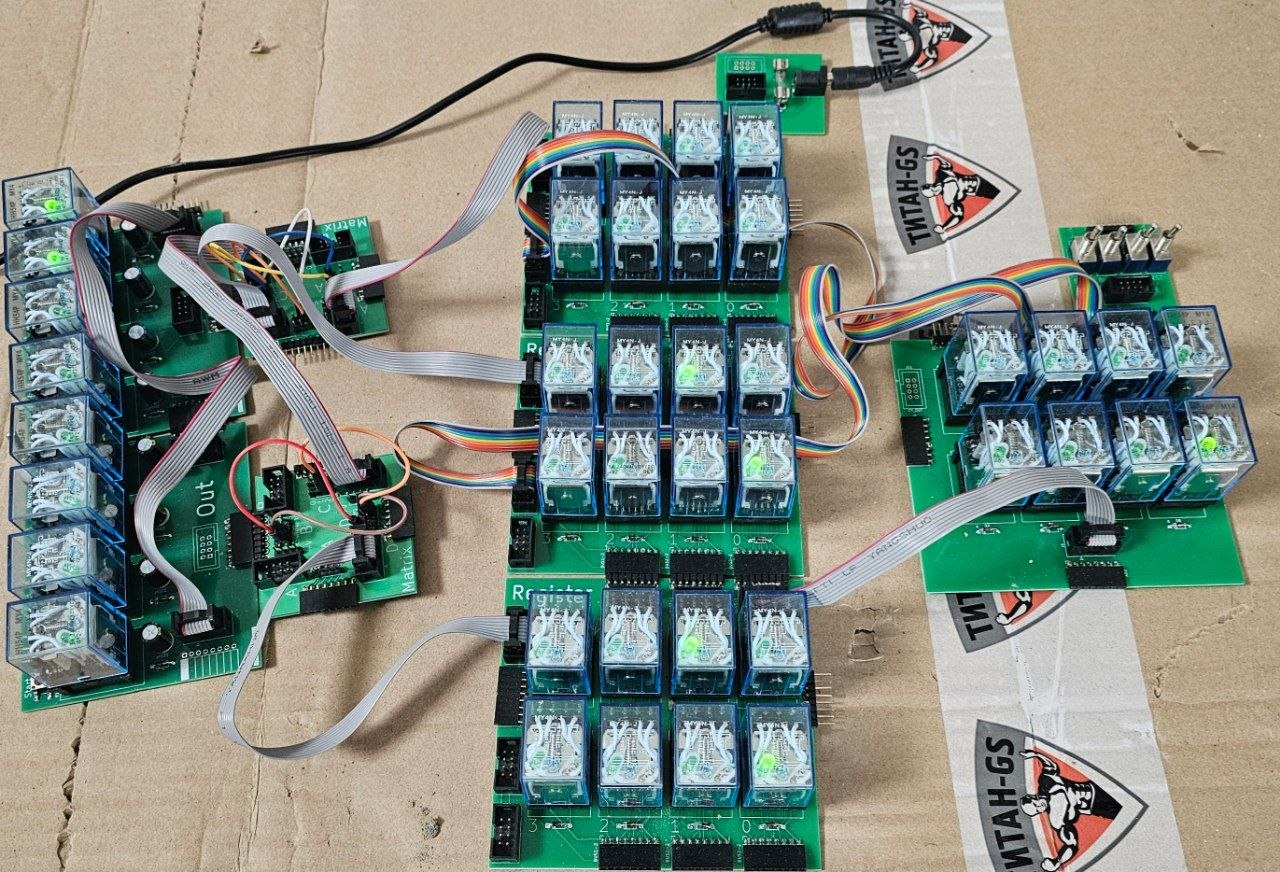
\includegraphics[width=0.5\columnwidth]{photo/fibonacci1.jpg}
\end{center}
